\documentclass{beamer}
\usetheme[hideothersubsections]{HRTheme}
\usepackage{beamerthemeHRTheme}
\usepackage{graphicx}
\usepackage[space]{grffile}
\usepackage{listings}
\lstset{language=SQL,
basicstyle=\ttfamily\footnotesize,
mathescape=true,
keywordstyle=\color{blue},
breaklines=true,
escapeinside={\%*}{*)}}
\usepackage[utf8]{inputenc}
\usepackage{color}
\newcommand{\red}[1]{
\textcolor{red}{#1}
}
\newcommand{\ts}{\textbackslash}

\title{Object-Relation Mapping}

\author{ }

\institute{Hogeschool Rotterdam \\ 
Rotterdam, Netherlands}

\date{}

\begin{document}
\maketitle

\SlideSection{Introduction}
\SlideSubSection{Lecture topics}
\begin{slide}{
\item Object-Relation Mapping.
\item Setting up Postgres.
\item Setting up hibernate.
}\end{slide}



\SlideSection{Object-Relation Mapping}
\SlideSubSection{JDBC}
\begin{slide}{
\item Provides a set of Java API for accessing the relational databases from Java program.
\item It allows querying/updating database data 
\item JDBC represents statements using one of the following classes:
\begin{enumerate}
	\pause
	 \item Statement – the statement is sent to the database server each and every time.
	 \pause
	 \item PreparedStatement – the statement is cached and then the execution path is pre-determined on the database server allowing it to be executed multiple times in an efficient manner.
	 \pause
	 \item CallableStatement – used for executing stored procedures on the database.
\end{enumerate}
}
\end{slide}



\SlideSubSection{Sample Code JDBC}
{
\begin{lstlisting}[language=java][showstringspaces=false]
..
try (Connection conn = DriverManager.getConnection(
	     "jdbc:somejdbcvendor:other data needed by some jdbc vendor",
	     "myLogin",
	     "myPassword" ) ) {
		
	Statement stmt = conn.createStatement()
	stmt.executeUpdate( "INSERT INTO Ships( name ) VALUE ( 'destroyer XYZ' ) " );
	}
 }  
..	
\end{lstlisting}	
}


\SlideSubSection{Disadvantages of JDBC}
\begin{slide}{
\item Less maintainable code for large projects
\item Queries are DBMS specific
}
\end{slide}

\SlideSubSection{ORM}
\begin{slide}{
\item It's a technique for converting data between relational databases and object-oriented programming languages.
\pause
\item Hides details of SQL queries from OO logic.
\pause
\item Based on JDBC 'under the hood'.
\pause 
\item Maps Java POJOs (plain old java objects) to relational databases
\pause 
\item Portability: DB independent
\pause 
\item Performance: Object and query caching mechanism 
}
\end{slide}


\SlideSubSection{ORM and Data Persistence Pattern}
\begin{slide}{
\item There are some pattern designed for persistence of objects in DBS
\item ORM framework are based on design patterns and framework specific implementations
\item Only two data persistence pattern will be discussed in this lecture
\pause 
\begin{itemize}
\item Active record pattern
\item Data mapper
\end{itemize}
}\end{slide}

\SlideSubSection{Active Record Pattern (ARP)}
\begin{slide}{
\item In ARP there is an object for every table or view that wraps a row
\item This object encapsulates the database access, and adds domain logic on that data
\pause
\item So this object carries both data and behavior 
}\end{slide}


\SlideSubSection{Active Record Pattern}
\begin{slide}{
\item sample structure of active record 
\\
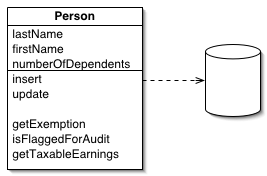
\includegraphics[scale=0.7]{img/activeRecordSketch.png}
}\end{slide}


\SlideSubSection{Active Record Pattern (ARP)}
\begin{slide}{
\item What are the limitations of this pattern regarding objects structure? 
\pause
\item Think of collections and inheritance! 
}\end{slide}


\SlideSubSection{Data Mapper Pattern (DMP)}
\begin{slide}{
\item In DMP there is a layer of mappers that moves data between objects and a database 
\item This layer keeps both in-memory objects and database independent from each others 
\item The reasons for this are:
\pause
\begin{itemize}
\item Objects and relational databases have different mechanisms for structuring data
\pause
\item Many parts of an object, such as collections and inheritance, aren't present in relational databases
\item Object schema and database schema do not match in many cases
\end{itemize}
}\end{slide}


\SlideSubSection{Data Mapper}
\begin{slide}{
\item sample structure of data mapper 
\\
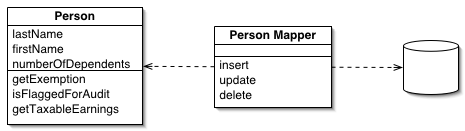
\includegraphics[scale=0.5]{img/databaseMapperSketch.png}
}\end{slide}



\SlideSubSection{Data Mapper Framework: Hibernate}
\begin{slide}{
\item Hibernate implements data mapper pattern
\item Components of Hibernate : 	
\begin{itemize}
\item Configuration file for the settings: hibernate.cfg.xml 
\pause
\item Mapping files for each entity: Entity.hbm.xml OR
\pause 
\item Annotiation in the POJO-files (@keyword in java files)
\pause
\item Hibernate Query Language (HQL) is an object-oriented query language
\end{itemize}
}\end{slide}


\SlideSubSection{Hibernate}
\begin{slide}{
\item sample structure of data mapper 
\\
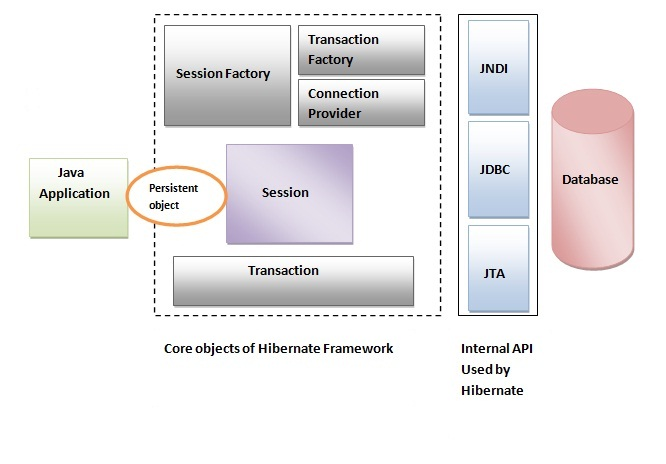
\includegraphics[scale=0.5]{img/Hibernate.jpg}
}\end{slide}

\begin{frame}[fragile]
Example of Hibernate configuration file 
\begin{lstlisting}[language=XML]
<?xml version="1.0" encoding="utf-8"?>
<!DOCTYPE hibernate-configuration SYSTEM 
"http://www.hibernate.org/dtd/hibernate-configuration-3.0.dtd">

<hibernate-configuration>
   <session-factory>
   <property name="hibernate.dialect">
      org.hibernate.dialect.PostgresSQLDialect
   </property>
   <property name="hibernate.connection.driver_class">
      com.postgres.jdbc.Driver
   </property>

   <!-- Assume test is the database name -->
   <property name="hibernate.connection.url">
      jdbc:mysql://localhost/test
   </property>
   <property name="hibernate.connection.username">
      root
   </property>
   <property name="hibernate.connection.password">
      root123
   </property>
   !-- List of XML mapping files -->
      <mapping resource="ships.hbm.xml"/>

   </session-factory>
   </hibernate-configuration>
\end{lstlisting}
\end{frame}

\begin{frame}[fragile]
POJO sample for Ships 
\begin{lstlisting}
public class Ships {
   private int serial;
   private String name; 
   private String armour;   
   ...
  public Ships() {}
   ...  
  }
 \end{lstlisting} 
\end{frame}

\begin{frame}[fragile]
Example of a mapping file in Hibernate
\begin{lstlisting}[language=XML]
<?xml version="1.0" encoding="utf-8"?>
<!DOCTYPE hibernate-mapping PUBLIC 
 "-//Hibernate/Hibernate Mapping DTD//EN"
 "http://www.hibernate.org/dtd/hibernate-mapping-3.0.dtd"> 

<hibernate-mapping>
   <class name="Ships" table="Ships">
      <meta attribute="class-description">
         This class contains the employee detail. 
      </meta>
      <id name="serial" type="int" column="serial">
         <generator class="native"/>
      </id>
      <property name="serial" column="serial" type="integer"/>
      <property name="name" column="name" type="string"/>
      <property name="armour" column="armour" type="integer"/>
   </class>
</hibernate-mapping>
\end{lstlisting} 
\end{frame}

\begin{frame}[fragile]
Example of using annotation instead of mapping files 
\begin{lstlisting}[language=java]
import javax.persistence.*;

@Entity
@Table(name = "ships")
public class Ships {
   @Id @GeneratedValue
   @Column(name = "serial")
   private int serial;

   @Column(name = "name")
   private String name;

   @Column(name = "armour")
   private String armour; 

   public Employee() {}
   \end{lstlisting} 
\end{frame}

\begin{frame}[fragile]
Sample code for persisting a new ship in Hibernate 
\begin{lstlisting}[language=java]
....	
Session session = factory.openSession();
      Transaction tx = null;
      Integer shipId = null;
      try{
         tx = session.beginTransaction();
         Ships s = new Ships("walle","metal armour");
         shipId = (Integer) session.save(Ships); 
         tx.commit();
      }catch (HibernateException e) {
         if (tx!=null) tx.rollback();
         e.printStackTrace(); 
      }finally {
         session.close(); 
      }
....
   \end{lstlisting} 
\end{frame}
 

\SlideSubSection{Java Persistence API}
\begin{slide}{
\item Provides the standard specification for managing the relational data in applications
\item JPA is a layer between third party ORM like Hibernate and the application 
\\
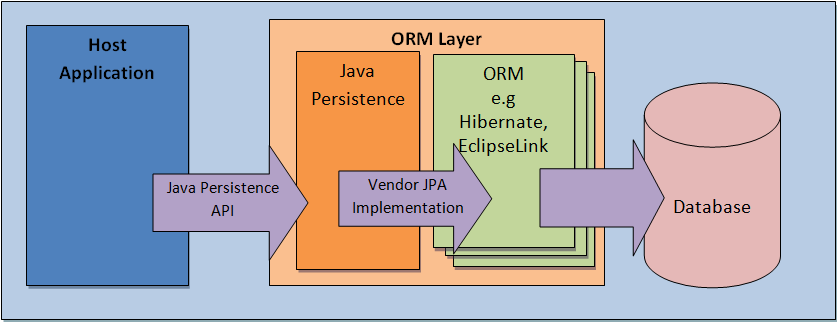
\includegraphics[scale=0.3]{img/JPA.png}
}
\end{slide} 
 

\SlideSubSection{Java Persistence API}
\begin{slide}{
\item Entities
\item EntityManager
\item Persistence Units
\item JPA Query Language
}
\end{slide}  

\begin{frame}[fragile]
Sample code for persisting a new ship in JPA with Hibernate 
\begin{lstlisting}[language=java]
....	 
EntityManagerFactory emf = Persistence.createEntityManagerFactory("InfDev5PU");
//create a session in case of Hibernate
EntityManager em = emf.createEntityManager();
//starts a transaction 
em.getTransaction().begin();
Ships s = new Ships("walle","metal armour");
//calls the save method of Hibernate
em.persist(em);
em.getTransaction().commit();
em.close();
....
\end{lstlisting} 
\end{frame} 
 

\SlideSubSection{Lab}
\begin{slide}{
\item Check the tables mentioned in les 0
\item Create these tables in Postgres
\item Insert new data into the database using Hibernate	
	}
\end{slide}

\end{document}
